\chapter{Arquitectura de la Fase 2}

La Fase 2 conserva la VPC \code{10.10.0.0/24} y los cinco segmentos implementados en la
fase anterior. El bloque de reserva \code{10.10.0.192/26} se divide en la DMZ
\code{10.10.0.192/27} y la reserva futura \code{10.10.0.224/27}. Esta división no modifica
ninguna dirección existente y mantiene 27 direcciones asignables para crecimiento.

\begin{figure}[H]
  \centering
  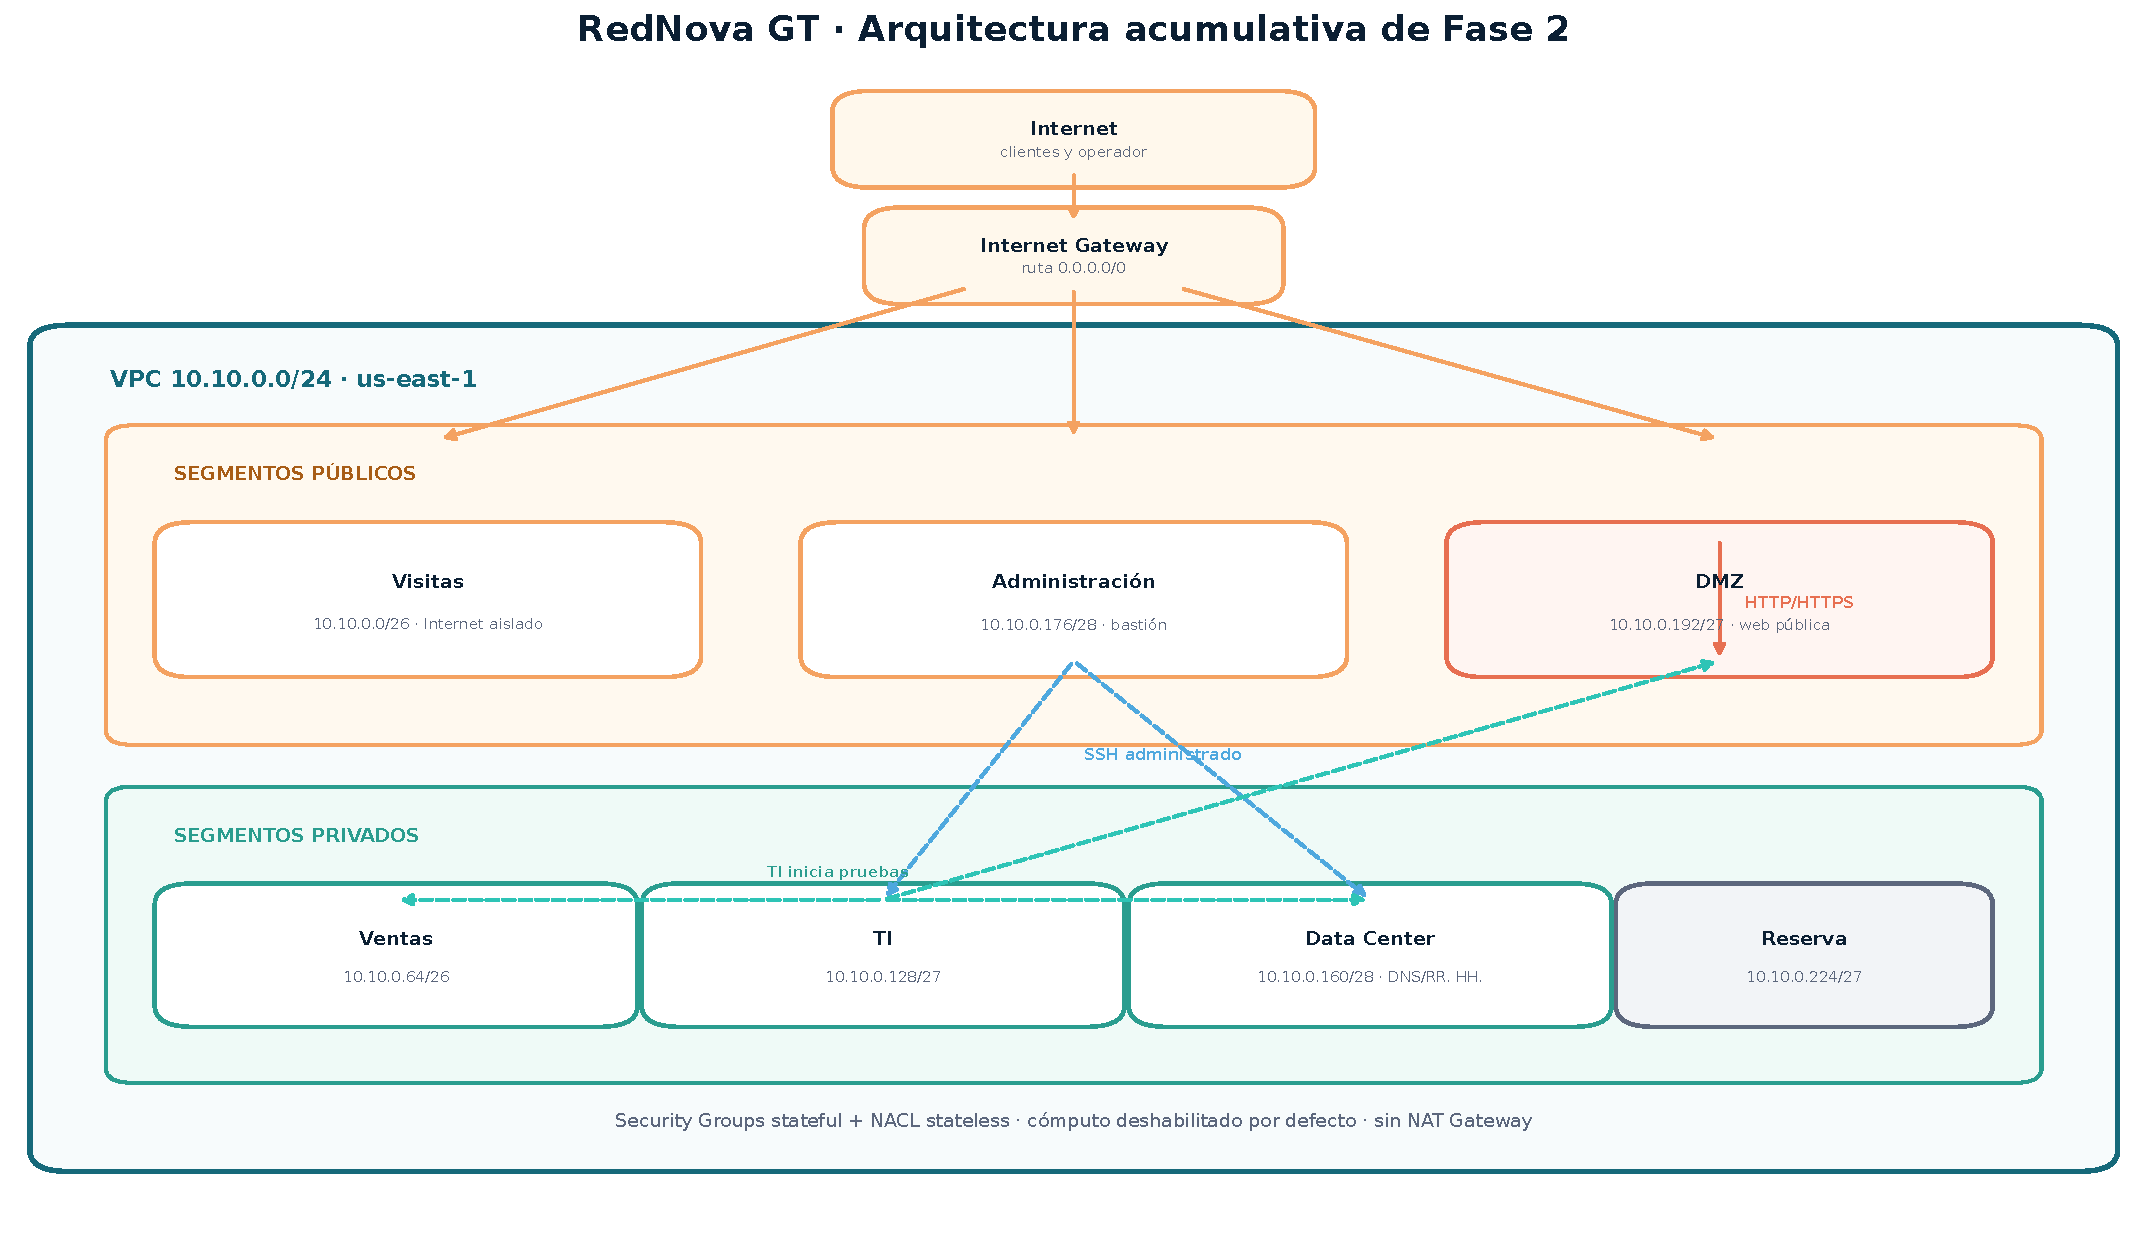
\includegraphics[width=\textwidth]{assets/diagrams/arquitectura-fase2.pdf}
  \caption{Arquitectura acumulativa con DMZ, rutas públicas y segmentos privados.}
\end{figure}

\begin{table}[H]
  \centering
  \caption{Direccionamiento acumulativo de la VPC}
  \begin{tabularx}{\textwidth}{@{}l l l Y@{}}
    \toprule
    Segmento & CIDR & Tipo & Uso \\
    \midrule
    Visitas & \code{10.10.0.0/26} & Pública & Cliente temporal con Internet aislado \\
    Ventas & \code{10.10.0.64/26} & Privada & Usuarios y pruebas heredadas \\
    TI & \code{10.10.0.128/27} & Privada & Administración y pruebas autorizadas \\
    Data Center & \code{10.10.0.160/28} & Privada & DNS e intranet de RR. HH. \\
    Administración & \code{10.10.0.176/28} & Pública & Bastión temporal \\
    DMZ & \code{10.10.0.192/27} & Pública & Web pública de Ventas \\
    Reserva & \code{10.10.0.224/27} & No asignada & Crecimiento futuro \\
    \bottomrule
  \end{tabularx}
\end{table}

La DMZ utiliza una tabla de rutas dedicada con \code{0.0.0.0/0} hacia el Internet Gateway.
La separación evita reutilizar implícitamente la tabla pública de Visitas y Administración y
permite auditar el segmento público de Ventas de forma independiente.

\begin{infobox}[Salida de Visitas]
Una ruta pública no asigna por sí sola una dirección IPv4 pública. Debido a que
\code{map_public_ip_on_launch} permanece deshabilitado, el cliente temporal de Visitas debe
recibir una IPv4 pública explícita durante la prueba. La dirección se retira al terminar la
ventana autorizada.
\end{infobox}

El diagrama fuente y la matriz completa de flujos se conservan en
\code{docs/fase-final/arquitectura-fase2.md}.
